\documentclass{intech}
 
%\usepackage{your_package}	%if you need custom package
%\usepackage[notquote]{hanging}
 

% * CHAPTER NUMBER * BOOK NAME * AUTHOR(S) NAME *****************************
\setcounter{chapter}{0} % It will be set by technical editor.

\booktitle{Wireless Energy Transfer  based on Electromagnetic Resonance: Principles and Engineering Explorations}%

\chaptertitle{The Phenomenon of Wireless Energy Transfer: Experiments and Philosophy} % You know your chapter title?

\authors{H. V\'azquez-Leal, A. Gallardo-Del-Angel, R. Casta\~neda-Sheissa and F. J. Gonz\'alez-Mart{\'i}nez}
\affiliation{Universidad Veracruzana \\ Facultad de Instrumentaci\'on Electr\'onica}
\country{M\'exico}

% uncomment the next three or six lines, when authors are from diferent university, company or country

%\secondauthors{Author(s) with another affiliation}
%\secondaffiliation{Name of the 2nd University (Company)}
%\secondcountry{2nd country}

%\thirdauthors{}
%\thirdaffiliation{}
%\thirdcountry{}

% END * CHAPTER NUMBER * BOOK NAME * AUTHOR(S) NAME *************************


\begin{document}

\maketitle

\section{Introducci\'on}

There is a basic law in thermodynamics; the law of conservation of energy, which states that {\it energy may neither be created nor destroyed just can be transformed}. Nature is an expert using this physics fundamental law favouring life and evolution of species all around the planet, it can be said that we are accustomed to live under this law that we do not pay attention to its existence and how it influence our lives.

Since the origin of the human kind, man has been using nature's energy in his benefit. When the fire was discovered the first thing tried was to transfer it where found to his shelter. Later on, man learned to gather and transport fuels like mineral charcoal, vegetable charcoal, among others, which then would be transformed into heat or light. In fact, energy transportation became so important for developing communities that when the electrical energy was invented, the biggest and sophisticated energy network ever known by the human kind was quickly built, that is, the electrical grid. Such distribution grid pushed great advances in science oriented to optimize the efficiency on driving such energy. Nevertheless, is common to loose around 30\% of energy due to several reasons. Nowadays, there are some daily life applications that could use an energy transport form without cables, some of them could be:

\begin{itemize}
\item Medical implants. The advance in biomedical science has allowed to create biomedical implants like: pacemakers, cochlear implants, subcutaneous drug supplier, among others.
\item Charge mobile devices, electrical cars, unmanned aircraft, to name a few.
\item Home appliances like irons, vacuum cleaners, televisions, etc.
\end{itemize}

Such potential applications promote the interest to use a wireless energy transfer.  Nevertheless, nature has always been a step beyond us, doing energy distribution and transformation since a long while without the need of copper cables. The biggest wireless transfer source known is solar energy; nature uses sunlight to drive the photosynthesis process, generating this way nutrients that later on will become the motor for the food chain and life. At present, several ways to turn sunlight into electrical power have been invented, among them, the photo-voltaic cells are the most famous. However, collecting solar energy is just the first step, the distribution of this energy is the other part of the problem, that is, the new objective is to wirelessly transfer point to point the energy.

This new technological tendency seeks towards wireless energy is not so new as one might think. It is already known that the true inventor of the radio was Nikola Tesla, therefore, makes sense to think that the same scientist to infer, if it was possible to transfer information using an electromagnetic field, it would be also possible to transfer power by the same mean. Thus, in the early 19nth century this prominent inventor and scientist performed experiments (\cite{RES20}) regarding the wireless energy transfer achieving astonishing results for his age. It has been said that Tesla's experiments achieved to light lamps about 40 Km away. Nevertheless, due to the dangerous nature of the experiments, low efficiency on power transfer, and mainly by the depletion of financial resources, Tesla abandoned experimentation, leaving his legacy in the form of a patent that was never commercially exploited.

Electromagnetic radiation has been typically used for the wireless transmission of information. However, information travels on electromagnetic waves which are a form of energy. Therefore, in theory it is possible to transmit energy similarly like the used to transfer information (voice and data). In particular, it is possible to transfer in a directional way great powers using microwaves (\cite{RES22}). Although the method is efficient, it has disadvantages: requires a line of sight and it is a dangerous mechanism for living beings. Thus, the wireless energy transfer using the phenomenon of electromagnetic resonance has become in a viable option, at least for short distances, since it has high efficiency for power transfer.

At present, energy has been transferred wirelessly using such diverse physical mechanisms like:

\begin{itemize}
\item Laser. The laser beam is coherent light beam capable to transport very high energies, this makes it in an efficient mechanism to send energy point to point in a line of sight. NASA (\cite{RES21}) introduced in 2003 a remote-controlled aircraft wirelessly energized by a laser beam and a photovoltaic cell infra-red sensitive acting as the energy collector. In fact, NASA is proposing such scheme to power satellites and wireless energy transfer where none other mechanism is viable (\cite{RES21}). 
\item Piezoelectric principle (\cite{RES8}). It has been demonstrated the feasibility to wirelessly transfer energy using piezoelectric transducers capable to emit and collect vibratory waves.
\item Radio waves and Microwaves. In \cite{RES22} is shown how to transmit high power energy through long distances using Microwaves. Also, there is a whole research field for rectennas \cite{RES4,RES9,RES10,RES12} which are antennas capable to collect energy from radio waves.
\item Inductive coupling (\cite{RES3,RES5,RES6,RES7}). The inductive coupling works under the resonant coupling effect between coils of two LC circuits. The maximum efficiency is only achieved when transmitter and receiver are placed very close from each other.
\item "Strong" electromagnetic resonance. In (\cite{RES1,RES2}) was introduced the method of wireless energy transfer, which use the "strong" electromagnetic resonance phenomenon, achieving energy transfer efficiently at several dozens of centimetres. 
\end{itemize}

Transferring great quantities of power using magnetic field creates, inevitably, unrest about the harmful effects that it could cause to human health. Therefore, the next section will address this concern.

\section{Electromagnetic Waves and Health}

Since the discovering of electromagnetic waves a technological race began to take advantage of transferring information wirelessly. This technological race started with Morse code transmission, but quickly came radio, television, cellular phones and the digital versions for all the mentioned previously. Adding to the mentioned before, in the last decade arrived an endless amount of mobile devices capable to communicate wirelessly, these are used massively around the globe. As a result, it is common that an average person is  subjected to magnetic fields in frequencies going from Megahertz up to the Gigahertz. Therefore, the concerts of the population about health effects due to be exposed to all the  electromagnetic radiation generated by our society every day. Besides, added to the debate is the concern for the wireless energy transfer mechanisms working with electromagnetic signals.

Several studies have been completed (\cite{RES15,RES16}) about the effects of electromagnetic waves, in particular for cellular phones, verifying that just at the upper international security levels some effects to genes are noticed. In (\cite{RES13}) is assured that it is not yet possible to determine health effects either on short or long terms due by the exposition to electromagnetic waves like the ones emitted by broadcasting stations and cellular networks. Nevertheless, in (\cite{RES14}) a study was performed to 10,497 marines from the Royal Norwegian Navy; the result for the ones who worked within 10 meters of broadcasting stations or radars, was an increase on infertility and a higher birth rate of women than men. This increase of infertility agrees with other study (\cite{RES14x}) that determined that the semen quality decay in men which by employment reasons (electricians, welders, technicians, etc.) are exposed to constant electromagnetic radiation including microwaves. The studies conclude that some effects on the human being in fact occur.

\section{Acoustic and Electrical Resonance}

The mechanical resonance or acoustic is well known on physics and consists in applying to an object a vibratory periodic action with a vibratory period that match the maximum absorption energy rate of the object. That frequency is known as resonant frequency. This effect may be destructive for some rigid materials like when a glass breaks when a tenor sings, or in more extreme cases even a bridge or a building may collapse due to resonance; whether it is caused by the wind or drums.


The phenomenon is well known in mechanics is also present in electricity and is called electrical resonance or inductive. Such phenomenon can be used to transfer wireless energy with two main advantages: maximum absorption rate is guaranteed and it can work in low frequencies (less dangerous to humans). When two objects have the same resonant frequency, they can be coupled in a resonant way causing one object to transfer energy (in an efficient way) to the other. This principle can be exploited to transmit energy from one point to another by means of an electromagnetic field. Next, three wireless energy transfer mechanisms are described:

\begin{enumerate}
\item {\bf Inductive coupling (\cite{RES3})} is a resonant coupling that takes place between coils of two $LC$ circuits with the same resonant frequency, transferring energy from one coil to the other as it can be seen in figure \ref{fuerte}. The disadvantage of this technique is that efficiency is lost as fast as coils are separated.
\item {\bf Self resonant coupling (\cite{RES1})}. The self resonance occur in a natural way for all coils ($L$), although the frequency ($f_r=1/(2\pi \sqrt{L C_p})$) is usually too high because the parasitic capacitance ($C_p$) value is too low. Nevertheless, in (\cite{RES1}) was shown that it is possible to achieve good efficiency with a scheme like the one shown in figure \ref{fuerte}(b). For the coupling to surpass the 40\% reported in \cite{RES1} the radius  ($r$) for the coil must be much lower than wavelength ($\lambda$) of the resonant frequency and the optimum separation ($d$) for a good coupling should be such $r\ll d\ll \lambda$, in such a way that the coupling is proportional to $(\frac{r}{\lambda}\frac{r^3}{d^3})$
(\cite{meta}). There are two fundamental differences for the simple inductive coupling in figure \ref{fuerte}(a), those are: the capacitance of the $LC$ circuit is parasite, not discrete, and now coils ($T$ y $R$) are coupled to two one spire coils $L_S$ and $L_L$, those act as the emitter source and receiver coils, respectively. The coil's self resonant frequency depends of its parasite capacitance, that is the reason the frequency is very high (around the GHz range). Therefore, to achieve lower self resonance frequency ($<10$Mhz) it is necessary to use thick and spaced copper wire to create higher parasite capacitance, reducing the self resonance frequency down to the megahertz range. In fact, in \cite{RES1} and \cite{RES2} is reported an experiment using cable with radius 3 cm. The efficiency on the power transfer with respect to the distance has an inverse relationship to the radius of the coil, that is why the experiments reported in \cite{RES1} and \cite{RES2} coils have 30 cm. radius.
\item In figure \ref{fuerte}(c), the coupling scheme shown can be named as {\bf strong resonant inductive coupling}, this is a modification for the strong resonant coupling (see figure \ref{fuerte}(b)). The modification consists in exchange the parasite capacitance $C_p$ for a discrete capacitance $C$. Thus, the need for large and thick cable is eliminated.
\end{enumerate}

\begin{figure}[htbp]	% H-must be here or [htb]
\centering
\subfigure[Inductive resonant coupling]{\includegraphics[width=7.3cm]{./img/acoplamientos-1.eps}} %	** if .eps don't need extension
\hspace{0.5cm}
\subfigure[Strong self-resonant coupling]{\includegraphics[width=7.7cm]{./img/acoplamientos-2.eps}}
\hspace{0.5cm}
\subfigure[Modified inductive resonant coupling]{\includegraphics[width=8cm]{./img/acoplamientos-3.eps}} %	** if .eps don't need extension
\vspace{-0.5cm}
\caption{Coupling schemes}
\label{fuerte}
\end{figure}

\section{Experimentation}

Triangular and circular coils are going to be employed in order to establish an inductive resonant coupling as shown in figure \ref{circutriangular}.

\begin{enumerate}
\item {\bf Inductive resonant coupling}. This experiment was designed (\cite{SOMI}) to visualize the radiation pattern and efficiency of an inductive resonant coupling. First, the generating coil was kept in a fixed position while the receiver coil ($R$) revolves around the generating coil ($T$), at a fixed distance and with constant angular displacement completing 360 degrees (see figure \ref{datos1}(a)). The experiment shows that the produced energy by the transmitter coil $T$ propagates at 90$^\circ$ in front of the generating coil and at 90$^\circ$ behind the same coil. In another stage of the experiment, two coils were placed in parallel and concentric at a distance of zero centimetres, then they were moved away. The results are shown in figure \ref{datos1}(c). It can be seen that the maximum efficiency for voltage gain is around the 50\% (at zero centimetres). The result is logical after observing  the radiation pattern shown in figure \ref{datos1}(b), because a radiation back lobe is wasted. Figure \ref{datos1}(c) shows, beyond the 8 centimetres distance, the voltage gain for the system falls below the 5\% value. The back lobe could be reused using a reflecting surface for the magnetic field.

\begin{figure}[htbp]	% H-must be here or [htb]
\centering
\subfigure[Experimental process for the revolving coil]{\includegraphics[width=7cm]{./img/coil3d.eps}} %	** if .eps don't need extension
\subfigure[Radiation pattern]{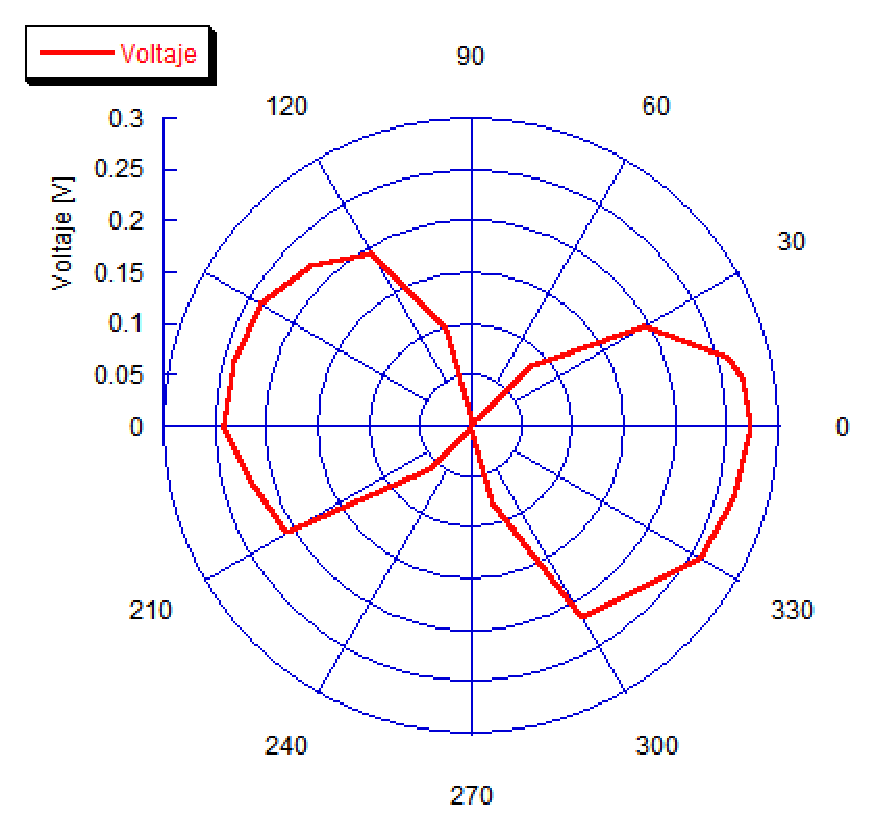
\includegraphics[width=7cm]{./img/image1a.eps}}
\subfigure[Voltage gain of the system with respect to the voltage ratio]{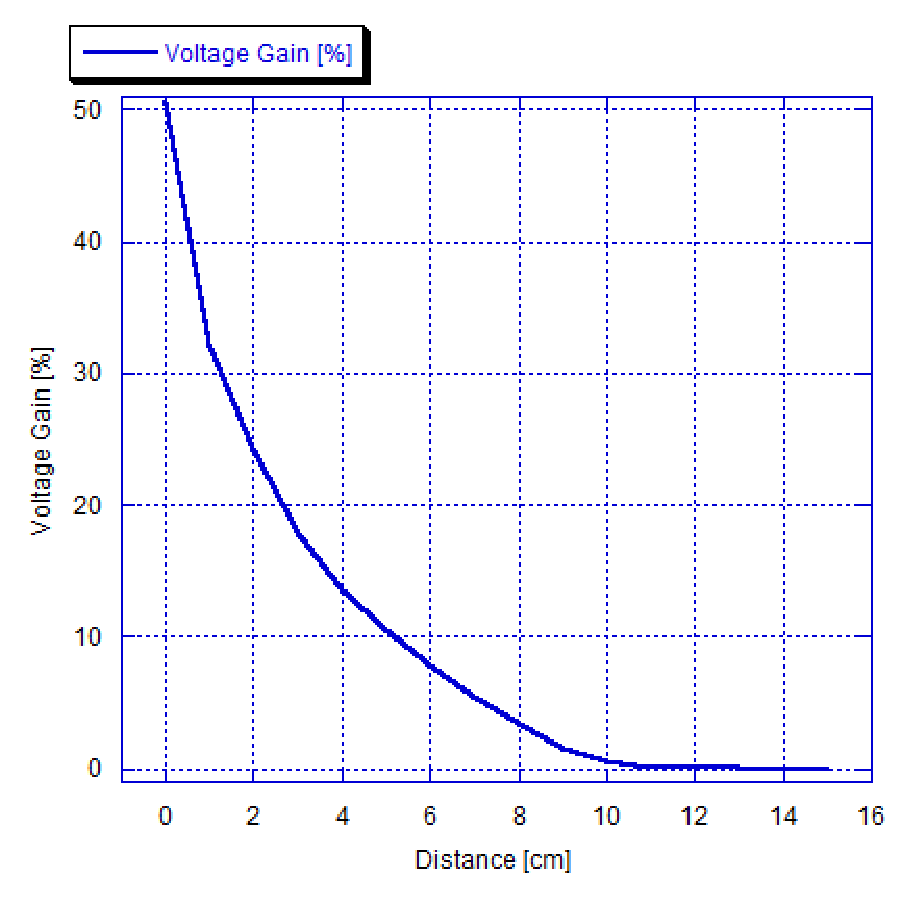
\includegraphics[width=6cm]{./img/image2.eps}} %	** if .eps don't need extension
\caption{Generator coil radiation pattern at 1.4 MHz.}
\label{datos1}
\end{figure}
\item {\bf Triangular coil}. 
\item  {\bf Modified resonant inductive coupling}. In the complete version of this work, the results will be presented.
On this experiment the previous procedure will be repeated, but the scheme employed is shown in figure \ref{fuerte}(c). The results obtained and the following discussion will be presented in the complete document, also a comparison to the experiment 1 will be included.
\item  {\bf Triangular coil}. At this moment preliminary results are being gathered and on review.  In the complete version of this work, the results will be presented.


\item {\bf Waveguide}. Experiments 1 and 2 will be repeated using a waveguide for the transmitter coil and a reflecting stage for the back lobe of the radiation pattern. The expected result is the achievement of higher efficiency at grater distance.
\end{enumerate}
\section{Philosophy}
The wireless energy with: high power (>100W), reaching longer distance (>10m), having good efficiency (>70\%), without health concerns, and low cost is a dream that keeps the attention of researchers around the planet. Nevertheless, in order to make a dream come true it is necessary innovating ideas or even radical ones, to provide the answer for the big questions opposed to achieve the goal. Therefore, innovation is required on the following directions:

\begin{itemize}
\item Coils with different geometries. Coils employed on the reported experiments are just a single spiral.  Nevertheless, new geometries (triangular, hexagonal, multiform) can be used and thus modify the radiation pattern, this modification on the pattern seeks the increase of: directionality, distance and/or efficiency. With completely different coils, like triangular, hexagonal, multiform, highly non-linear radiation patterns could be generated like the ones shown in figure \ref{patronloco}.
\begin{figure}[hbtp]
\centering
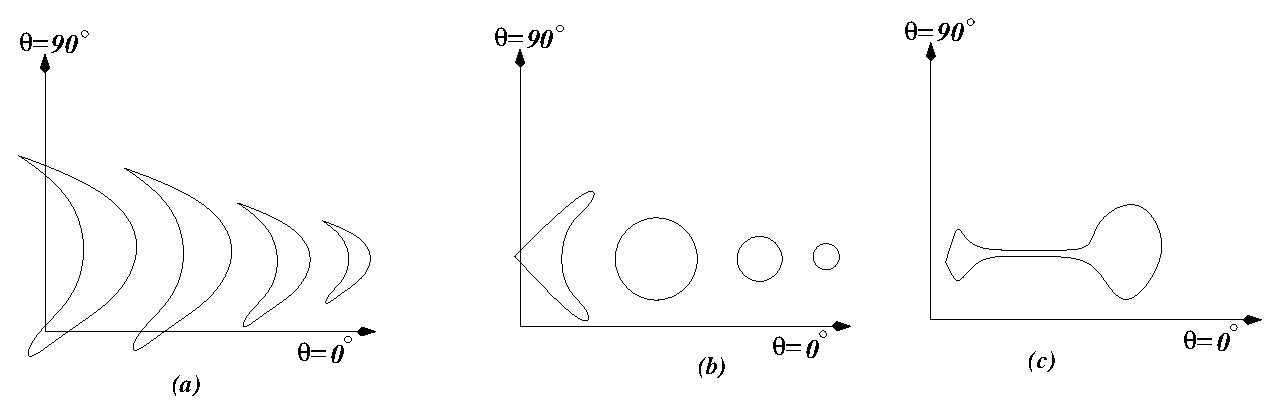
\includegraphics[width=12cm]{img/patrones.eps}
\caption{New radiation patterns.}
\label{patronloco}
\end{figure}



\item Using new materials to improve efficiency. For instance, from the self-resonance coils in experiment 2, it can be achieved using a coil-capacitor device. This coil could be designed in such a way that between each spire a dielectric material is placed to create parasite capacitance along all the coil spires. Therefore, parasite capacitance will be big enough to achieve self-resonance on the order of MHz. The advantage of this coil-capacitor is that no longer thick coils and spaced spires will be needed.
\item In (\cite{meta} was demonstrated that using metamaterials could improve performance of coupled resonant systems in near field. They proposed a power relay system based on a near-field metamaterial superlens. This is the first step toward optimization of the resonant coupling phenomenon in near field, the next will be the design of coils implemented with metamaterials looking to affect directionality or efficiency.
\item Inductive coupled multi-resonant systems. Using amorphous or multiform coils could generate multiple resonant frequencies that could be employed in the transfer of energy using more than one resonant frequency, this will depend on their emitting pattern and efficiency extent. Another possible application for multi-resonant systems is transmission of energy and information a the same time using different channels. For instance, using the information channel to establish the permission for the energy transfer and features like power levels.
\item {\bf Waveguide}. A waveguide designed for the transmitter coild and a reflecting stage in order to use the back lobe of the radiation pattern, may help to improve efficiency of the power transfer.
\end{itemize}



\bibliography{lrc}

\end{document}
